\documentclass[a4paper, 11pt]{article}

\usepackage[utf8x]{inputenc}
\usepackage[T1]{fontenc}
\usepackage{ucs}
\usepackage[english]{babel}
\usepackage{mathtools, amsmath, amsfonts}
\usepackage{fancyhdr}
\usepackage[parfill]{parskip}
\usepackage{palatino,newtxmath}
\usepackage{float}
\usepackage[font={small,it}]{caption}
\usepackage{minted}
\usepackage{graphicx, float}

\linespread{1.05}
\pagestyle{fancyplain}
\fancyhead{}
\fancyfoot[L]{}
\fancyfoot[C]{}
\fancyfoot[R]{\thepage}
\renewcommand{\headrulewidth}{0pt}
\renewcommand{\footrulewidth}{0pt}
\setlength{\headheight}{13.6pt}

\widowpenalty=1000
\clubpenalty=1000

\newcommand{\horrule}[1]{\rule{\linewidth}{#1}}

\title{ 
\normalfont \normalsize 
\textsc{University of Copenhagen} \\ [25pt]
\horrule{0.5pt} \\[0.4cm]
\huge XMP: Assignment 2 \\ \Large - Programming \\
\horrule{2pt} \\[0.5cm]
}

\author{Jens Fredskov (chw752)}

\begin{document}
\maketitle
\pagebreak

\section{Implementation} % (fold)
\label{sec:implementation}

The implementation consists of several different processes, one for rooms, one for a player, a controller giving instructions to the player. The controller is either a shell or an ai. The processes communicate as shown in Figure \ref{fig:communication}

\begin{figure}[H]
    \centering
   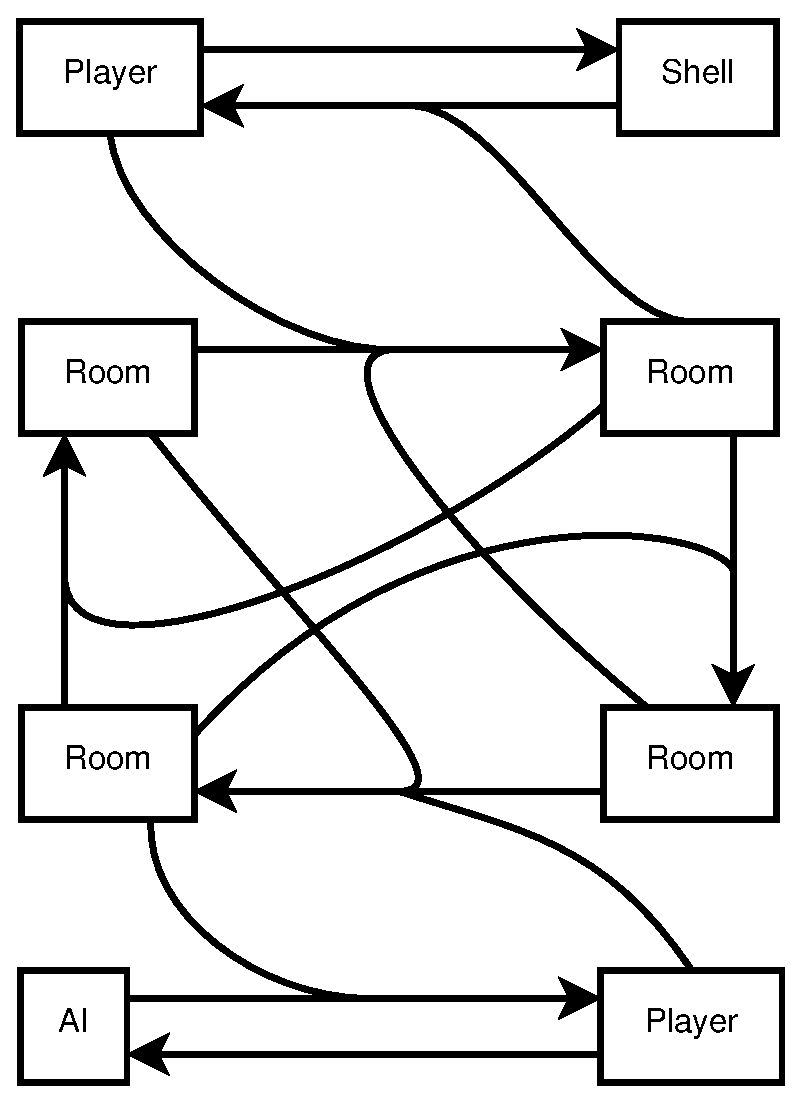
\includegraphics[width=0.5\textwidth]{communication.eps}
   \caption{An example of a dungeon with four rooms and two players (one human and one ai).}
\label{fig:communication}
\end{figure}

Rooms are instantiated with a channel for requests, a map of channels which should be other rooms request channel, a map of items in the room and a map of players currently in the room. The room listens on its request channel in a loop and handles requests from either players or other rooms. The latter happens when a player goes from one room to another.

Players are instantiated with a channel for requests, a response channel for its controller, a channel for waiting on room responses, the request channel of the room in which the player currently is. The player listens on its request channel, which can come from either a controller or a room. The latter happens when another player moves to a room a which point the room sends a message to all players already in the room.

Controllers are instantiated with a channel for sending requests to a player and a channel for receiving responses. To allow messages about players entering the same room as you to appear the controller for humans (i.e. the shell) starts its input as a process and waits on either input or responses on the response channel.

To properly kill all processes the shell takes an extra parameter, an ordered list of request channels. This allows it to send ``exit''-requests to rooms and players in a specified order. When a player exits it closes the response channel of its controller. If the controller is an ai it just shuts down. If it is a shell it instead runs through its list of channels and shuts down these processes. The ai should be shut down before any rooms.

% section implementation (end)

\appendix
\section{Source code} % (fold)
\label{sec:source_code}

\inputminted[fontsize=\scriptsize, frame=topline, label=main.go, linenos=true]{go}{../src/main.go}

\inputminted[fontsize=\scriptsize, frame=topline, label=xmpmud/structs.go, linenos=true]{go}{../src/xmpmud/structs.go}

\inputminted[fontsize=\scriptsize, frame=topline, label=xmpmud/controller.go, linenos=true]{go}{../src/xmpmud/controller.go}

\inputminted[fontsize=\scriptsize, frame=topline, label=xmpmud/player.go, linenos=true]{go}{../src/xmpmud/player.go}

\inputminted[fontsize=\scriptsize, frame=topline, label=xmpmud/room.go, linenos=true]{go}{../src/xmpmud/room.go}
% section source_code (end)

\end{document}